\documentclass[10pt, landscape]{article}
\usepackage[scaled=0.92]{helvet}
\usepackage{calc}
\usepackage{multicol}
\usepackage{ifthen}
\usepackage[a4paper,margin=5mm,landscape]{geometry}
\usepackage{amsmath,amsthm,amsfonts,amssymb}
\usepackage{color,graphicx,overpic}
\usepackage{hyperref}
\usepackage{newtxtext} 
\usepackage{enumitem}
\usepackage{amssymb}
\usepackage[table]{xcolor}
\usepackage{vwcol}
\usepackage{tikz}
\usetikzlibrary{arrows.meta}
\usetikzlibrary{calc}
\usepackage{mathtools}
\usepackage{nicematrix}
\usepackage[T1]{fontenc} %%% <--- NOTE THIS
% for relations
\usepackage{cancel}
\usepackage{ mathrsfs }
\usepackage{listings}
\usepackage{background}
\setlist{nosep}

\usepackage{etoolbox}
\makeatletter
\preto{\@verbatim}{\topsep=0pt \partopsep=0pt }
\makeatother

\backgroundsetup{
scale=1,
color=black,
opacity=0.4,
angle=0,
contents={%
  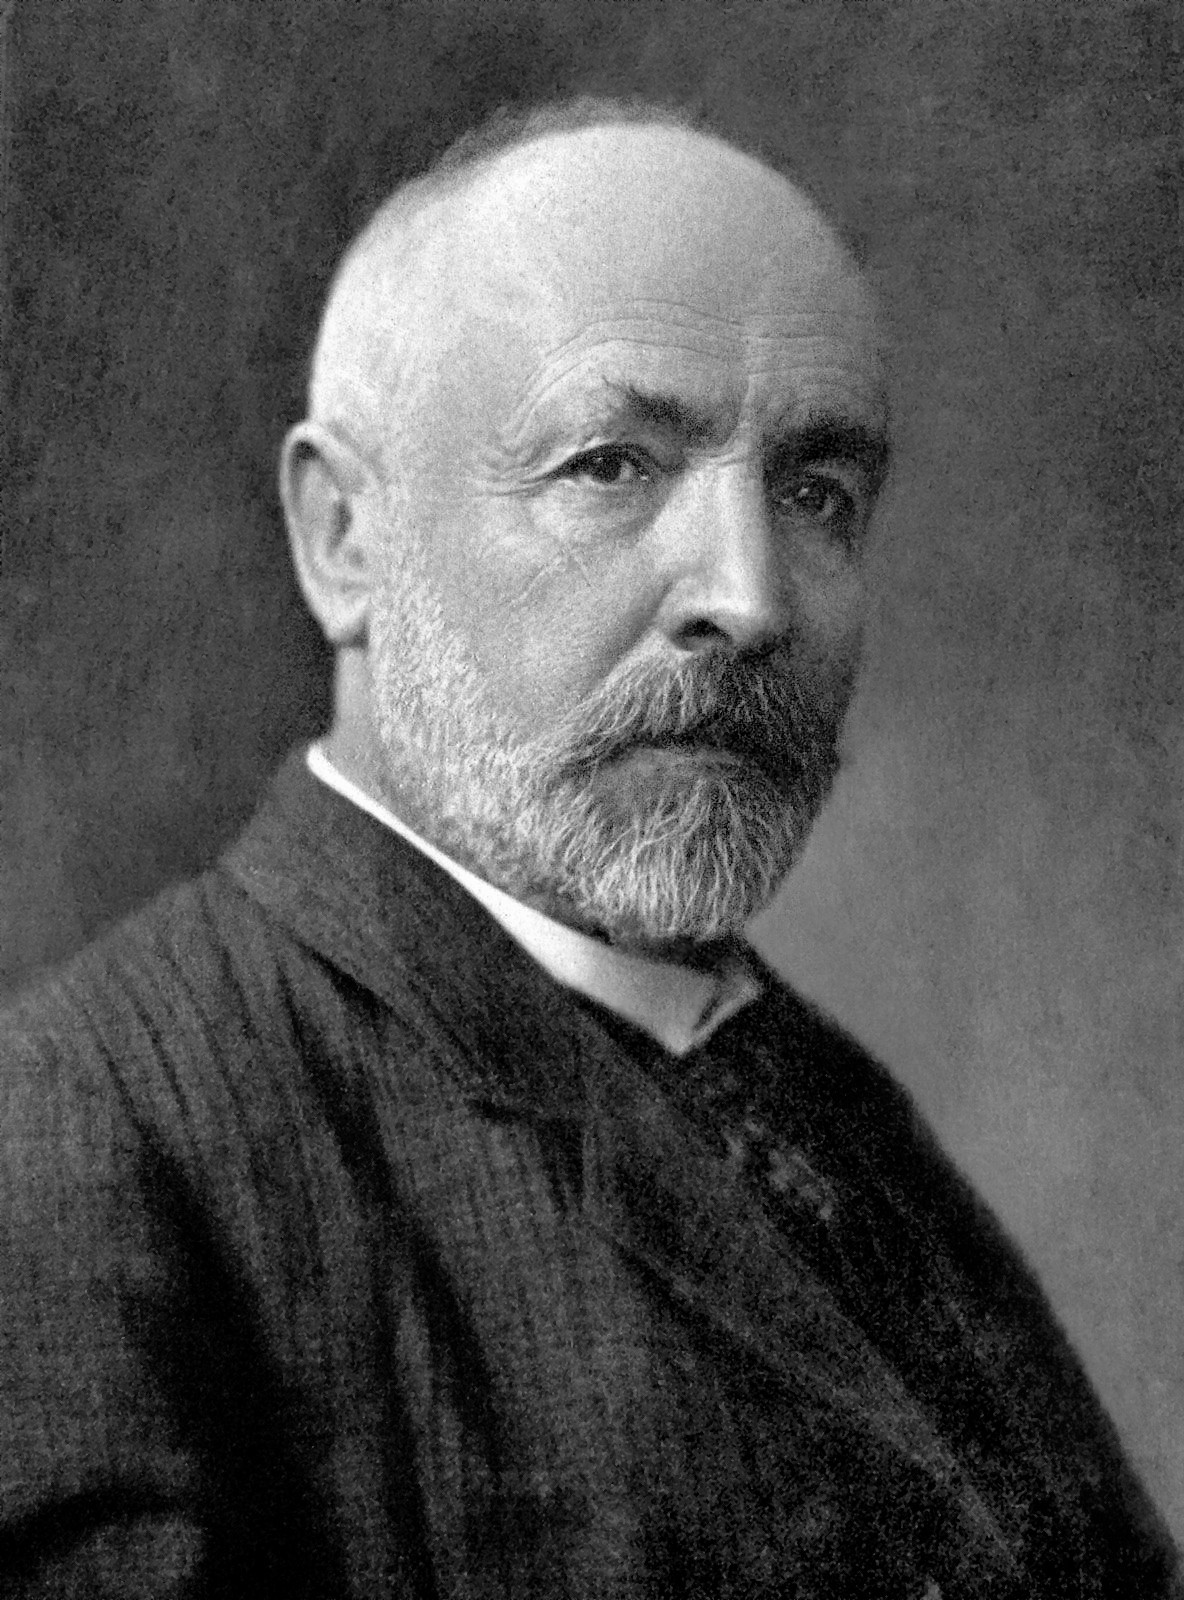
\includegraphics[width=0.5\paperwidth,height=\paperheight]{cantor.jpg}
  
\includegraphics[width=0.5\paperwidth,height=\paperheight]{dilip.jpg}
  }%
}

\pdfinfo{
  /Title (MA3205.pdf)
  /Creator (TeX)
  /Producer (pdfTeX 1.40.0)
  /Author (Seamus)
  /Subject (Example)
  /Keywords (pdflatex, latex,pdftex,tex)}

\lstset{language=Java,keywordstyle={\bfseries \color{black}}}

% Turn off header and footer
\pagestyle{empty}

\newenvironment{tightcenter}{%
  \setlength\topsep{0pt}
  \setlength\parskip{0pt}
  \begin{center}
}{%
  \end{center}
}

% redefine section commands to use less space
\makeatletter
\renewcommand{\section}{\@startsection{section}{1}{0mm}%
                                {-1ex plus -.5ex minus -.2ex}%
                                {0.5ex plus .2ex}%x
                                {\normalfont\large\bfseries}}
\renewcommand{\section}{\@startsection{section}{2}{0mm}%
                                {-1explus -.5ex minus -.2ex}%
                                {0.5ex plus .2ex}%
                                {\normalfont\normalsize\bfseries}}
\renewcommand{\subsection}{\@startsection{subsection}{3}{0mm}%
                                {-1ex plus -.5ex minus -.2ex}%
                                {1ex plus .2ex}%
                                {\normalfont\small\bfseries}}%
\renewcommand{\familydefault}{\sfdefault}
\renewcommand\rmdefault{\sfdefault}
% makes nested numbering (e.g. 1.1.1, 1.1.2, etc)
\renewcommand{\labelenumii}{\theenumii}
\renewcommand{\theenumii}{\theenumi.\arabic{enumii}.}
\renewcommand\labelitemii{•}
%  for logical not operator
\renewcommand{\lnot}{\mathord{\sim}}
\renewcommand{\bf}[1]{\textbf{#1}}
\newcommand{\abs}[1]{\vert #1 \vert}
\newcommand{\Mod}[1]{\ \mathrm{mod}\ #1}

\makeatother
\definecolor{myblue}{cmyk}{1,.72,0,.38}
\everymath\expandafter{\the\everymath \color{myblue}}
% Define BibTeX command
\def\BibTeX{{\rm B\kern-.05em{\sc i\kern-.025em b}\kern-.08em
    T\kern-.1667em\lower.7ex\hbox{E}\kern-.125emX}}
\let\iff\leftrightarrow
\let\Iff\Leftrightarrow
\let\then\rightarrow
\let\Then\Rightarrow

% Don't print section numbers
\setcounter{secnumdepth}{0}

\setlength{\parindent}{0pt}
\setlength{\parskip}{0pt plus 0.5ex}
%% this changes all items (enumerate and itemize)
\setlength{\leftmargini}{0.5cm}
\setlength{\leftmarginii}{0.5cm}
\setlist[itemize,1]{leftmargin=2mm,labelindent=1mm,labelsep=1mm}
\setlist[itemize,2]{leftmargin=4mm,labelindent=1mm,labelsep=1mm}

%My Environments
\newtheorem{example}[section]{Example}
% -----------------------------------------------------------------------

\begin{document}
\raggedright
\footnotesize
\begin{multicols*}{3}

% multicol parameters
% These lengths are set only within the two main columns
\setlength{\columnseprule}{0.25pt}
\setlength{\premulticols}{1pt}
\setlength{\postmulticols}{1pt}
\setlength{\multicolsep}{1pt}
\setlength{\columnsep}{2pt}

\begin{center}
    \fbox{%
        \parbox{0.8\linewidth}{\centering \textcolor{black}{
            {\Large\textbf{MA3205}}
            \\ \normalsize{AY24/25 Sem 2}}
            \\ {\footnotesize \textcolor{myblue}{by ngmh}} 
        }%
    }
\end{center}

\section{2. Pairing, Products, and Relations}
\textbf{EP2.36} There is a bijection $F:\mathcal{P}(X)\rightarrow \{0,1\}^X$. 
$F(a)(x) =
    \left\{
    \begin{array}{lr}
      0 & \text{if $x \in A$} \\
      1 & \text{if $x \notin A$} \\
    \end{array}
    \right.
$ which is $1-1$ and onto.

\textbf{D2.37 Cartesian Product} Let $F$ be a function with $dom(F)$ as a set. $\prod F=\{f:f \ \text{is a function} \land dom(f) = dom(F) \land \forall x \in dom(F) \ [f(x) \in F(x)]\}$. If $F=\langle A_i : i \in I \rangle$, then $\prod F = \prod_{i \in I}A_i = \{f: f \ \text{is a function} \land dom(f)=I \land \forall i \in I\ [f(i) \in A_i]\}$

\textbf{A2.38 Axiom of Choice} If $\langle A_i : i \in I \rangle$ is a sequence of sets such that $\forall i \in I \ [A_i \neq \emptyset]$, then $\prod_{i \in I} A_i \neq \emptyset$

\section{4. The Natural Numbers}
\textbf{D4.17 Extenders} Let $\mathbf{FN}=\{\sigma:\sigma \ \text{is a function}\land \exists n \in \mathbb{N} \ [dom(\sigma)=n]\}$ be the proper class of all functions whose domain is some natural number. An extender is a function $\mathbf{E:FN\rightarrow V}$. When you input $\sigma=\{\langle 0, \sigma(0) \rangle, ...,\langle n, \sigma(n) \rangle\}$ into $\mathbf{E}$, $\mathbf{E}(\sigma)$ outputs the next value $\sigma(S(n))$.

\textbf{D2.45 Addition}
\begin{itemize}
    \item Define $\langle f_m : m \in \mathbb{N} \rangle$ such that $f_m: \mathbb{N} \rightarrow \mathbb{N}$ is the unique function such that $f_m(0)=m$ and $\forall n \in \mathbb{N} \ [f_m(S(n))=S(f_m(n))]$
    \item In other words, define the extender $\mathbf{E:FN\rightarrow V}$ as follows. For any $\sigma \in \mathbf{FN}$, $\mathbf{E}(\sigma) =
    \left\{
    \begin{array}{lr}
      m & \text{if $dom(\sigma)=0$} \\
      S(\sigma(\bigcup dom(\sigma))) & \text{if $dom(\sigma) \neq 0$} \\
    \end{array}
    \right.
    $
    \item $f_m:\mathbb{N}\rightarrow \mathbf{V}$ is the unique function satisfying $\forall n \in \mathbb{N} \ [f_m(n)=\mathbf{E}(f_m \restriction n)]$.
    \item Then $m+n=f_m(n)$, and $m + S(n) = (m+n)+1$.
\end{itemize}

\section{5. Comparing Sizes of Sets}
\textbf{D5.1 Equinumerosity} $A \approx B$ if there exists $f:A \rightarrow B$ which is both $1-1$ and onto.

\textbf{F5.2} $\mathcal{P}(A)\approx\{0, 1\}^A$

\textbf{D5.4} $A \lessapprox B$ means there exists $f:A \rightarrow B$ which is $1-1$ and $B$ is at least as big as $A$. If $A \lessapprox B$ but $A \not\approx B$, then $A \lnapprox B$. It is not possible to find $g : A \rightarrow B$ that is both $1-1$ and onto. $B$ is strictly bigger in size than $A$.

\textbf{L5.5} If $f:A \rightarrow B$ and $g:B \rightarrow C$ are $1-1$ functions then $g \circ f : A \rightarrow C$ is $1-1$.

\textbf{L5.6} For sets $A,B,C$
\begin{enumerate}
    \item $A \lessapprox A$
    \item If $A \lessapprox B$ and $B \lessapprox C$ then $A \lessapprox C$
    \item If $A \approx B$ and $B \approx C$ then $A \approx C$
\end{enumerate}

\textbf{T5.7 Cantor} For any set $X$, $X \lnapprox \mathcal{P}(X)$.

\subsection{5.2 The Schröder Bernstein Theorem}
\textbf{T5.11 Schröder-Bernstein} For any sets $A$ and $B$, if $A \lessapprox B$ and $B \lessapprox A$, then $A \approx B$.

\textbf{E5.12} Suppose $f:X \rightarrow Y$ is a $1-1$ function. For any $Z \subseteq X$, $Z \approx Im_f(Z)$.

\textbf{E5.13} Suppose $I \subseteq A$ and $J \subseteq B$. If $I \approx J$ and $(A \ \backslash \ I) \approx (B \ \backslash \ J)$, then $A \approx B$.

\textbf{E5.14} If $n \in \mathbb{N}$ and $A \approx S(n)$, then $\forall a \in A, ( A \ \backslash \ \{a\} \approx n)$.

\textbf{E5.15} If $n \in \mathbb{N}$ and $A \approx n$, then if $a \notin A$, $(A \cup \{a\}) \approx S(n)$.

\textbf{E5.16} Let $n, m \in \mathbb{N}$. Then
\begin{enumerate}
    \item If $f:n \rightarrow n$ is $1-1$, then $f$ is onto. There is no $1-1$ function from $S(n)$ to $n$.
    \item If $m \in n$, then $m \lnapprox n$.
    \item If $x \subsetneq n$, then $x \lnapprox n$.
    \item $n \lnapprox \mathbb{N}$
    \item If $A \approx n$, $B \approx m$, and $A \cap B = \emptyset$, then $(A \cup B) \approx (n+m)$.
\end{enumerate}

\textbf{D5.19} A set is finite if there exits $n \in \mathbb{N}$ such that $n \approx A$. $A$ is infinite if it is not finite. $A$ is countable if $A \lessapprox \mathbb{N}$. $A$ is uncountable if it is not countable.

\textbf{L5.20} If $f:A\rightarrow B$ is a $1-1$ function, then for any $X,Y\subseteq A$, if $Im_f(X)=Im_f(Y)$, then $X=Y$.

\textbf{L5.21} For sets $A,B,C,D$
\begin{enumerate}
    \item If $A \lessapprox B$ then $\mathcal{P}(A) \lessapprox \mathcal{P}(B)$
    \item If $A \lessapprox B$ then $A^C \lessapprox B^C$
    \item If $A \lessapprox B, C \lessapprox D,$ and $B \cap D = \emptyset$, then $A\cup C \lessapprox B \cup D$
\end{enumerate}

\textbf{L5.22} If $n \in \mathbb{N}$ and $A \lessapprox n$, then $A$ is finite.

\textbf{L5.23} If $n \in \mathbb{N}$ and there exists an onto function $\sigma : n \rightarrow A$, then $A \lessapprox n$

\textbf{L5.24} If $A$ and $B$ are finite, then so is $A \cup B$.

\textbf{T5.25} If $A$ is a finite set and $f$ is a function with $dom(f)=A$ then
\begin{enumerate}
    \item If $X \subsetneq A$, then $X \lnapprox A$
    \item $ran(f)$ is finite and $ran(f) \lessapprox A$
    \item If $\forall a \in A \ [a \text{ is finite}]$ then $\cup A $ is finite
    \item $\mathcal{P}(A)$ is finite
\end{enumerate}

\textbf{E5.26} If $A \subseteq \mathbb{N}$ is finite and nonempty, $max(A)=\bigcup A$

\textbf{E5.27} If $A \lessapprox C$ and $B \lessapprox D$, then $A \times B \lessapprox C \times D$. If $A$ and $B$ are finite, $A \times B$ and $A^B$ are finite.

\textbf{E5.28} If $I$ is a finite set and $\langle A_i:i \in I \rangle$ is a sequence of sets such that $\forall i \in I \ [A_i \text{ is finite}]$, then $\prod_{i \in I} A_i$ is finite.

\textbf{E5.30} For any function, $dom(f) \approx f$.

\section{6. Orders}
\subsection{Quasi, Partial, Linear, and Well-Orders}
\textbf{D6.2 Quasi Order} Reflexive, Transitive
\begin{enumerate}
    \item $\forall x \in X \ [x \leq x]$
    \item $\forall x, y, z \in X \ [(x \leq y \land y \leq z) \Rightarrow x \leq z]$
\end{enumerate}

\textbf{D6.4 Partial Order} Irreflexive, Transitive
\begin{enumerate}
    \item $\forall x \in X \ [x \not < x]$
    \item $\forall x, y, z \in X \ [(x < y \land y < z) \Rightarrow x < z]$
\end{enumerate}

\textbf{D6.5 Linear Order} Irreflexive, Transitive, Comparable
\begin{enumerate}
    \item $\forall x \in X \ [x \lhd x]$
    \item $\forall x, y, z \in X \ [(x \lhd y \land y \lhd z) \Rightarrow x \lhd z]$
    \item $\forall x, y \in X \ [x = y \lor x \lhd y \lor y \lhd x]$
\end{enumerate}

\textbf{F6.6} Suppose $\langle X, < \rangle$ is a partial order. Define a relation $\leq$ on $X$ by $x \leq y$ iff $x < y$ or $x = y$. Then $\langle X, \leq \rangle$ is a quasi order where $\forall x, y \in X \ [(x \leq y \land y \leq x) \Rightarrow x = y]$.

\textbf{C6.8} If $\langle X, < \rangle$ is a partial order and $Y \subseteq X$ then $(Y \times Y) \ \cap <$ is a partial order on $Y$, as a shorthand for $\langle Y, ((Y \times Y)\ \cap <)\rangle$. Restricted to $Y$ then $Z$ is the same as restricting directly to $Z$.

\textbf{D6.9 Maximal / Minimal Element} $x \in X$ is maximal if $\forall y \in X \ [x \not < y]$. $x \in X$ is minimal if $\forall y \in X \ [y \not < x]$. There could be multiple in a partial order.

\textbf{L6.10} A finite non-empty partial order has both a maximal and minimal element.

\textbf{D6.11} $C \subseteq X$ is a chain if $\forall x, y \in C \ [x \text{ and } y \text{ are comparable}]$. $A \subseteq X$ is an antichain if $\forall x, y \in A \ [x \neq y \Rightarrow x \text{ and } y \text{ are incomparable}]$. A chain is maximal if there is no chain $C' \subseteq X$ where $C \subsetneq C'$. $\emptyset$ and singletons are chains and antichains.

\textbf{L6.12} For a finite partial order, every chain or antichain is contained in a maximal chain or antichain.

\textbf{D6.13 Well-Order} Every non-empty subset has a minimal element. $\forall A \subseteq X \ [A \neq \emptyset \Rightarrow \exists a \in A \ \forall a' \in A \ [a \leq a']]$.

\textbf{L6.15 (AC)} A linear order $\langle X, < \rangle$ is a well-order iff there is no $f : \mathbb{N} \rightarrow X$ where $\forall n \in \mathbb{N} \ [f(n) > f(n+1)]$.

\textbf{D6.16} For a linear order $\langle X, < \rangle$ $pred_{\langle X, < \rangle}(x)=\{x' \in X : x' < x\}$, or the set of predecessors of $x$ in $X$ for the ordering $<$. A subset $A \subseteq X$ is downwards closed if $\forall a \in A \ \forall x \in X \ [x < a \Rightarrow x \in A]$. The predecessor subset is downwards closed along with the entire set.

\textbf{F6.17} For a linear order $\langle X, < \rangle$, if $A \subseteq X$ is downwards closed, $\forall a \in A \ pred_{\langle A, < \rangle}(a)=pred_{\langle X, < \rangle}(a)$.

\textbf{F6.19} Let $\langle X, < \rangle$ be a well-order and $A$ a downwards closed subset of $X$. Etiher $A=X$ or $\exists x \in X$ such that $A = pred_{\langle X, < \rangle}(x)$.

\textbf{E6.20} If $\langle X, < \rangle$ is a well-order and $A \subseteq X$, $\langle A, < \rangle$ is a well-order.

\textbf{E6.21} Let $\langle X, < \rangle$ be a linear order. $f: X \rightarrow X$ is expansive if $\forall x \in X\ [f(x) \geq x]$, and order-preserving if $\forall x, y \in X \ [x < y \Rightarrow f(x) < f(y)]$. If $\langle X, < \rangle$ is a well-order, every order-preserving $f$ is expansive.

% \textbf{E6.22} Suppose $\langle X, < \rangle$ is a quasi-order. Define $E$ on $X$ by $\forall x, y \in X$, $x\ E\ y$ iff $x \leq y$ and $y \leq x$. $E$ is an equivalence relation on $X$. Let $Z=\{[x] : x \in X\}$ where $[x]$ is the equivalence class of $x$ under $E$. Define $\prec$ on $Z$ by $[x] \prec [y]$ iff $x \leq y$ and $y \not \leq x$. This relation is well-defined and a partial order on $Z$.

\subsection{New orders from old}
\textbf{L6.23} Suppose $X$ is a set and $\langle Y, \prec \rangle$ and $\langle Z, \lhd \rangle$ are partial orders. Suppose $f: X \rightarrow Y$ and $g : X \rightarrow Z$ are functions. Define $<$ on $X$ by stipulating that $\forall x, x' \in X$, $x < x' \leftrightarrow (f(x) \prec f(x')\ or \ (f(x) = f(x') \ and \ g(x) \lhd g(x')))$. Then,
\begin{enumerate}
    \item $<$ is a partial order on $X$
    \item if $\langle Y, \prec \rangle$ and $\langle Z, \lhd \rangle$ are both linear orders and $\forall x, x' \in X \ [(f(x) = f(x') \ and \ g(x) = g(x')) \Rightarrow x = x']$ then $<$ is also a linear order on $X$
    \item similarly for well-orders
\end{enumerate}

\textbf{C6.24} Let $X$ be a set and $\langle Y, \prec \rangle$ be a partial order. Suppose $f: X \rightarrow Y$ is a function. Define $<^*$ on $X$ by $\forall x, x' \in X$, $x <^* x' \leftrightarrow f(x) \prec f(x')$. Then $<^*$ is a partial order on $X$. If $f$ is $1-1$ and $\prec$ is a linear order on $Y$, then $<^*$ is a linear order on $X$. Similarly for well-orders. Use $Y = Z$, $f = g$, $\prec=\lhd$.

\textbf{EP 6.25 Lexographic / Dictionary Order} Define $f : \mathbb{N} \times \mathbb{N} \rightarrow \mathbb{N}$ and $g : \mathbb{N} \times \mathbb{N} \rightarrow \mathbb{N}$ by setting $f(\langle m, n \rangle)=m$ and $g(\langle m, n \rangle)=n$ for all $\langle m, n \rangle \in \mathbb{N} \times \mathbb{N}$. By L6.23, the relation $<_{lex}$ defined on $\mathbb{N} \times \mathbb{N}$ by $\langle m, n \rangle <_{lex} \langle k, l \rangle \leftrightarrow (f(\langle m, n \rangle)  \in f(\langle k, l \rangle)\ or \ (f(\langle m, n \rangle) = f(\langle k, l \rangle) \ and \ g(\langle m, n \rangle)  \in g(\langle k, l \rangle))) \leftrightarrow (m \in k \ or \ (m = k \ and \ n \in l))$ is a well-order on $\mathbb{N} \times \mathbb{N}$.

\textbf{D6.26} Suppose $\langle I, < \rangle$ is a well-order and $X$ is a set. For $f, g \in X^I$, if $f \neq g$, define $\Delta(f, g) = min(\langle \{i \in I : f(i) \neq g(i)\}, <\rangle)$. It is well-defined for the conditions mentioned above.

\textbf{L6.27} Suppose $\langle X, \lhd \rangle$ is a linear order and $\langle I, < \rangle$ is a well-order. Define $\prec$ on $X^I$ $\forall f, g \in X^I$ by $f \prec g \leftrightarrow (f \neq g \ and \ f(\Delta(f, g)) \lhd g(\Delta(f, h)))$. Then $\prec$ is a linear order on $X^I$.

\textbf{D6.28}
\begin{itemize}
    \item $[\mathbb{N}]^n=\{a \in \mathcal{P}(\mathbb{N}) : a \approx n\}$, or subsets of the naturals equinumerous to $n$.
    \item $\mathbb{N}^n=\{\sigma : \sigma \text{ is a function and } dom(\sigma)=n \land ran(\sigma) \subseteq \mathbb{N}\}$, or functions with domain $n$ and range as a subset of the naturals.
    \item $[\mathbb{N}]^{<\omega}=\{a \in \mathcal{P}(\mathbb{N}): a \text{ is finite}\}$, or subsets of the naturals equinumerous to finite $n$.
    \item $\mathbb{N}^{<\omega} = \{\sigma : \sigma \text{ is a function and } dom(\sigma)\in \mathbb{N} \land ran(\sigma) \subseteq \mathbb{N}\}$, or functions with a finite domain and range as a subset of naturals.
    \item $[\mathbb{N}]^{<\omega}=\bigcup_{n \in \mathbb{N}}[\mathbb{N}]^n$ and $\mathbb{N}^{<\omega}=\bigcup_{n \in \mathbb{N}}\mathbb{N}^n$.
\end{itemize}

\textbf{EP6.29} $\langle \mathbb{N}, \in \rangle$ is a well-order. Define a linear order $<_{lex}$ on $\mathbb{N}^\mathbb{N}$ using L6.27. Since $2^\mathbb{N} \subseteq \mathbb{N}^\mathbb{N}$, $\langle 2^\mathbb{N}, <_{lex}\rangle$ is also a linear order. Define $F:\mathbb{N}^{<\omega} \rightarrow \mathbb{N}^\mathbb{N}$ as follows. $\sigma \in \mathbb{N}^{<\omega}$, $dom(\sigma)\in\mathbb{N}$ and $\sigma:dom(\sigma)\rightarrow \mathbb{N}$. Define $F(\sigma):\mathbb{N}\rightarrow\mathbb{N}$ by $F(\sigma)(n) =
    \left\{
    \begin{array}{lr}
      \sigma(n) & \text{if $n \in dom(\sigma)$} \\
      dom(\sigma) & \text{if $n \notin dom(\sigma)$} \\
    \end{array}
    \right.
    $
for every $n \in \mathbb{N}$. $F$ is $1-1$. Since $<_{lex}$ is a linear order on $\mathbb{N}^\mathbb{N}$, by C6.24, $<_{lex}$ defined on $\mathbb{N}^{<\omega}$ by $\sigma <_{lex} \tau \leftrightarrow F(\sigma) <_{lex} F(\tau)$ is also a linear order. From EP2.36, we have a $1-1$ and onto $F:\mathcal{P}(\mathbb{N})\rightarrow2^\mathbb{N}$. We can induce $A <_{lex} B \leftrightarrow F(A) <_{lex} F(B)$ for $A, B \in \mathcal{P}(\mathbb{N})$. Since $[\mathbb{N}]^{<\omega}\subseteq\mathcal{P}(\mathbb{N})$, $\langle [\mathbb{N}]^{<\omega}, <_{lex} \rangle$ is also a linear order.

\textbf{E6.30} Let $\langle X, < \rangle$ and $\langle Y, \prec \rangle$ be partial orders. Define $\langle X \times Y, \lhd \rangle$ by $\langle x, y \rangle \lhd \langle x', y' \rangle \leftrightarrow (x < x' \land y \prec y')$. This is a partial order.

\textbf{E6.31} A linear order $\langle X, < \rangle$ is dense if $\forall x, z \in X$ with $x < z$, $\exists y \in X$ such that $x < y < z$. $\langle \mathbb{N}^\mathbb{N}, <_{lex} \rangle$ is dense while $\langle 2^\mathbb{N}, <_{lex} \rangle$ is not dense.

\textbf{E6.32} $<_{lex}$ on $\mathcal{P}(\mathbb{N})$ is defined by the $1-1$ and onto $F$ from $EP2.36$.
\begin{enumerate}
    \item $\forall A, B \in \mathcal{P}(\mathbb{N})$, $A <_{lex} B$ iff $A \neq B \land min(A \ 
    \triangle \ B) \in A$
    \item $\langle [\mathbb{N}]^{<\omega} \backslash \{\emptyset\}, <_{lex} \rangle$ does not have any maximal or minimal elements
    \item $\langle [\mathbb{N}]^{<\omega} \backslash \{\emptyset\}, <_{lex} \rangle$ is dense
\end{enumerate}

\subsection{6.3 Embeddings and Isomorphisms}
\textbf{D6.33} If $\langle X, \lhd \rangle$ and $\langle Y, \prec \rangle$ are linear orders, $f: X \rightarrow Y$ is an isomorphism between them if $f$ is $1-1$ and onto and $\forall x, y \in X \ [x \lhd y \Leftrightarrow f(x) \prec f(y)]$. Two linear orders are isomorphic if $f$ exists which is an isomorphism.

\textbf{L6.34} $\langle X, \lhd \rangle$ and $\langle Y, \prec \rangle$ are linear orders. Suppose $f:X \rightarrow Y$ is an onto function such that $\forall x, y \in X \ [x \lhd y \Rightarrow f(x) \prec f(y)]$. $f$ is an isomorphism.

\textbf{D6.35} $\langle X, < \rangle$ and $\langle Y, \prec \rangle$ are linear orders. $f:X\rightarrow Y$ is an embedding if $\forall x, x' \in X \ [x < x' \Leftrightarrow f(x) \prec f(x')]$ and $f$ is $1-1$.  If there exists and embedding $f$, we say that $\langle X, < \rangle$ embeds into $\langle Y, \prec \rangle$ and $\langle X, <\rangle \hookrightarrow \langle Y, \prec \rangle$. $\langle X, < \rangle$ is isomorphic to $\langle Im_f(X), \prec \rangle$.

\textbf{F6.36} $\langle X, < \rangle$ and $\langle Y, \prec \rangle$ are linear orders. If $f: X \rightarrow Y$ is a function such that $\forall x, x' \in X \ [x < x' \Rightarrow f(x) \prec f(x')]$, then $f$ is an embedding.

\textbf{F6.37} $\langle X, < \rangle$ and $\langle Y, \prec \rangle$ are linear orders. Suppose $A$ and $B$ are downwards closed subsets of $X$ and $Y$. If $f: A \rightarrow B$ is an isomorphism from $\langle A, < \rangle$ to $\langle B, \prec \rangle$, then $\forall a \in A, f\restriction pred_{\langle X, < \rangle}(a)$ is an isomorphism from $\langle pred_{\langle X, < \rangle}(a), < \rangle$ to $\langle pred_{\langle Y, \prec \rangle}(f(a)), \prec \rangle$.

\textbf{T6.38} Suppose $\langle X, \lhd \rangle $ is a finite linear order. $\exists! n \in \mathbb{N}$ such that $\langle X, \lhd \rangle $ is isomorphic to $\langle n, \in \rangle$. This isomorphism is unique.

\textbf{T6.39} Suppose $\langle X, \lhd \rangle$ is an infinite linear order such that $\forall x \in X, pred_{\langle X, \lhd \rangle}$ is finite. $\langle X, \lhd \rangle$ is isomorphic to $\langle \mathbb{N}, \in \rangle$. The isomorphism from $X$ to $\mathbb{N}$ is unique.

\textbf{CL6.40} $\forall x, y \in X \ [x \lhd y \Rightarrow f(x) \in f(y)]$.

\textbf{CL6.41} $ran(f)$ is a downwards closed subset of $\langle \mathbb{N}, \in \rangle$.

\textbf{D6.42} A linear order $\langle X, \lhd \rangle$ has type omega $\omega$ if $X$ is infinite and $\forall x \in X$, $pred_{\langle X, \lhd \rangle}(x)$ is finite.

\section{7. Countable and Uncountable Sets}
\subsection{Countable Sets}
\textbf{C7.1} If $X \subseteq \mathbb{N}$ is infinite, $\langle X, \in \rangle$ is isomorphic to $\langle \mathbb{N}, \in \rangle$.

\textbf{C7.2} If $X$ is infinite and countable, then $X \approx \mathbb{N}$.

\textbf{T7.3} There exist linear orders of type omega on $\mathbb{N} \times \mathbb{N}$, $[\mathbb{N}]^{<\omega}$, and $\mathbb{N}^{<\omega}$. Define $f : \mathbb{N}\rightarrow X$ to show infinite, then $g: X \rightarrow \mathbb{N}$ and $h : X \rightarrow X$. Define $\prec$ as normal, and use it to show $pred_{\langle X, \prec\rangle}(x)$ is finite.

\textbf{C7.4}
\begin{enumerate}
    \item $\mathbb{N} \times \mathbb{N} \approx \mathbb{N}$, $[\mathbb{N}]^{<\omega} \approx \mathbb{N}$, and $\mathbb{N}^{<\omega} \approx \mathbb{N}$
    \item $\forall n \in \mathbb{N} \ [n \geq 1 \Rightarrow \mathbb{N}^n \ \land [\mathbb{N}]^{<\omega} \approx \mathbb{N}]$
\end{enumerate}

\textbf{L7.5} Suppose that $\langle A_n: n \in \mathbb{N} \rangle$ and $\langle f_n : n \in \mathbb{N} \rangle$ are sequences such that $\forall n \in \mathbb{N}$, $f_n: A_n \rightarrow \mathbb{N}$ is $1-1$. Then $\bigcup_{n \in \mathbb{N}} A_n$ is countable.

\textbf{L7.6 (AC)} A countable union of countable sets is countable. If $\langle A_n : n \in \mathbb{N} \rangle$ is a sequence of countable sets, then $\bigcup_{n \in \mathbb{N}}A_n$ is countable.

\textbf{L7.8} The set of rationals $\mathbb{Q}$ is countable, i.e. $\mathbb{Q} \rightarrow \mathbb{N}$.

\textbf{E7.9} Let $\langle X, < \rangle$, $\langle Y, \lhd \rangle$ and $\langle Z, \prec \rangle$ be linear orders. Suppose $f: X \rightarrow Y$ and $g: Y \rightarrow Z$ are isomorphisms. $f^{-1} : Y \rightarrow X$ and $g \circ f : X \rightarrow Z $ also are.

\textbf{E7.10} Define a sequence of relations $\langle \lhd_n : n \in \mathbb{N} \rangle$ by induction on $n \in \mathbb{N}$. Let $\lhd_0$ be $\emptyset$. Suppose $\lhd_n$ is a relation on $[\mathbb{N}]^n$. Define $\lhd_{n+1}$ as follows. Fix $a, b \in [\mathbb{N}]^{S(n)}$. If $max(a) < max(b)$, $a \lhd_{n+1} b$. If $max(a) = max(b)$, $a \cap max(b)$ and $b \cap max(b)$ are in $[\mathbb{N}]^n$. Then if $a \cap max(a) \lhd_n b \cap max(b)$, $a \lhd_{n+1} b$. Now define $\langle \prec_n : n \in \mathbb{N} \rangle$ by induction. $\prec_0=\emptyset$. Suppose $\lhd_n$ is a relation on $\mathbb{N}^n$. Define $\prec_{n+1}$ as follows. Fix $\sigma, \tau \in \mathbb{N}^{n+1}$. $ran(\sigma)$ and $ran(\tau)$ are finite non-empty subsets of $\mathbb{N}$. If $max(ran(\sigma)) < max(ran(\tau))$, $\sigma \prec_{n+1} \tau$. $\sigma \restriction n$ and $\tau \restriction n$ are members of $\mathbb{N}^n$. If $max(ran(\sigma))=max(ran(\tau))$ and if $\sigma \restriction n \prec_n \tau \restriction n$, then $\sigma \prec_{n+1} \tau$. If $max(ran(\sigma))=max(ran(\tau))$, $\sigma \restriction n = \tau \restriction n$, and $\sigma(n) < \tau(n)$, then $\sigma \prec_{n+1} \tau$. 
\begin{enumerate}
    \item $\langle \lhd_n : n \in \mathbb{N} \rangle$ is well-defined, $\forall n \in \mathbb{N}$, $\langle [\mathbb{N}]^n, \lhd_n \rangle$ is a linear order of type $\omega$.
    \item $\langle \prec_n : n \in \mathbb{N} \rangle$ is well-defined, $\forall n \in \mathbb{N}$, $\langle \mathbb{N}^n, \prec_n \rangle$ is a linear order of type $\omega$.
    \item We can then prove $(2)$ and $(3)$ of T7.3 without AC.
\end{enumerate}

\textbf{E7.11} Extenders for the following:
\begin{enumerate}
    \item $f(0)=f(1)=1$, $f(n)=f(n-1)+f(n-2) \ \forall n > 1$ $\mathbf{E}(\sigma) =
    \left\{
    \begin{array}{lr}
      1 & \text{$dom(\sigma) \in 2\}$} \\
      \sigma(\bigcup dom(\sigma))+\sigma(\bigcup \bigcup dom(\sigma)) & \text{for valid $dom(\sigma)$ etc.} \\
      \emptyset & \text{otherwise} \\
    \end{array}
    \right.
    $
    \item $f(n)=\lhd_n$ on $[\mathbb{N}]^n$
    % $\mathbf{E}(\sigma) =
    % \left\{
    % \begin{array}{lr}
    %   \emptyset & \text{$dom(\sigma) =0$} \\
    %   \{\langle s, t \rangle \in [\mathbb{N}]^{dom(\sigma)} \times [\mathbb{N}]^{dom(\sigma)} : [(\bigcup s)\in(\bigcup t)]\ or  & dom(\sigma) \neq 0 \\
    %   [(\bigcup s)=(\bigcup t)\ and\ \langle s \cap (\bigcup s), t \cap (\bigcup t)\rangle \in \sigma(\bigcup dom(\sigma))]\} & dom(\sigma) \neq 0 \\
    % \end{array}
    % \right.
    % $
    \item $f(n)=\prec_n$ on $\mathbb{N}^n$
    \begin{center}
        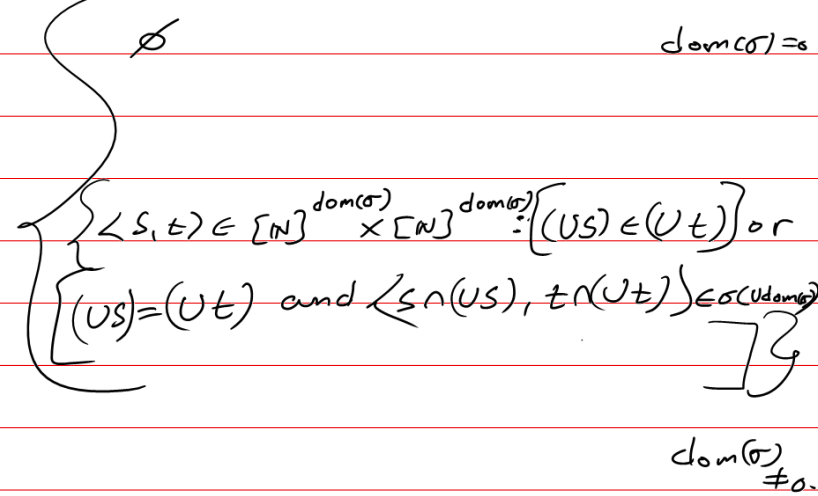
\includegraphics[width=0.49\linewidth]{extender1.png}    
        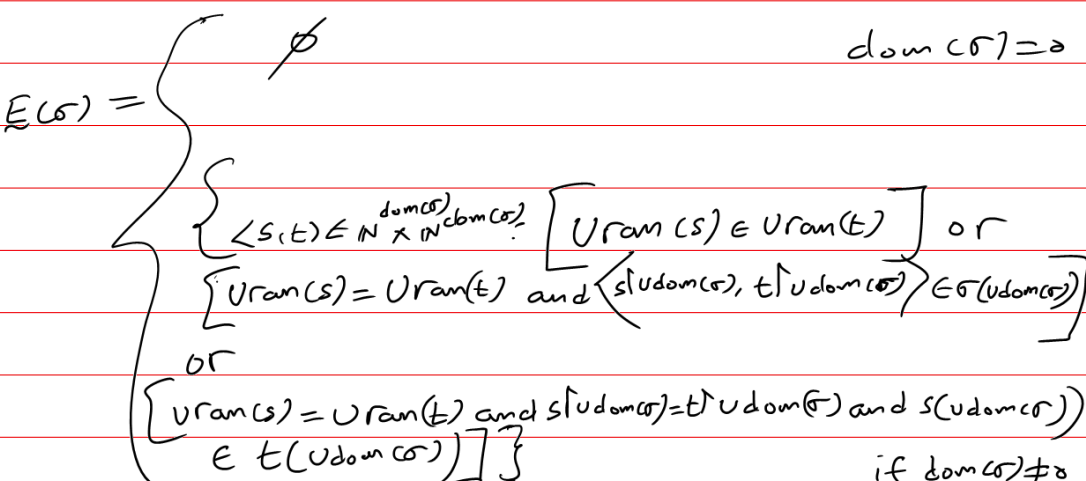
\includegraphics[width=0.49\linewidth]{extender2.png}    
    \end{center}
\end{enumerate}


\subsection{7.2 Sets of Size Continuum}
\textbf{F7.12} If $x, y \in \mathbb{R}$ and $x < y$, there is a $q \in \mathbb{Q}$ with $x < q < y$.

\textbf{L7.13} $2^\mathbb{N} \lessapprox \mathbb{R} \lessapprox \mathcal{P}(\mathbb{Q})$

\textbf{T7.14} These sets are equinumerous: $2^\mathbb{N}$, $\mathbb{N}^\mathbb{N}$, $\mathcal{P}(\mathbb{N} \times \mathbb{N})$, $\mathcal{P}(\mathbb{N})$, $\mathcal{P}(\mathbb{Q})$, $\mathbb{R}$. $2^\mathbb{N} \subseteq \mathbb{N}^\mathbb{N} \subseteq \mathcal{P}(\mathbb{N} \times \mathbb{N})$. So $2^\mathbb{N} \lessapprox \mathbb{N}^\mathbb{N} \lessapprox \mathcal{P}(\mathbb{N} \times \mathbb{N})$. $\mathbb{N} \approx \mathbb{N} \times \mathbb{N}$. By L5.22, $\mathcal{P}(\mathbb{N})\lessapprox \mathcal{P}(\mathbb{N} \times \mathbb{N}) \lessapprox \mathcal{P}(\mathbb{N})$ so $\mathcal{P}(\mathbb{N}) \approx \mathcal{P}(\mathbb{N} \times \mathbb{N})$. By L7.8, $\mathbb{Q} \lessapprox \mathbb{N}$. By F5.2, $2^\mathbb{N} \lessapprox \mathbb{R} \lessapprox \mathcal{P}(\mathbb{Q}) \lessapprox \mathcal{P}(\mathbb{N}) \lessapprox 2^\mathbb{N}$. We also have $2^\mathbb{N} \lessapprox \mathbb{N}^\mathbb{N} \lessapprox \mathcal{P}(\mathbb{N} \times \mathbb{N}) \lessapprox 2^\mathbb{N}$.

\textbf{D7.15} A set $X$ has size continuum or size $\mathfrak{c}$ if $X \approx \mathcal{P}(\mathbb{N})$.

\textbf{L7.16} $(r, s)=\{x \in \mathbb{R} : r < x < s\}$ has size $\mathfrak{c}$. The function $f(x) =
    \left\{
    \begin{array}{lr}
      \frac{x-t}{s-x} & \text{if $x \geq t$} \\
      \frac{x-t}{x-r} & \text{if $x < t$} \\
    \end{array}
    \right.
    $ is well-defined and $1-1$ and onto.

\textbf{E7.17} Let $l \subseteq \mathbb{R}^2$ be a line. Define $\phi:\mathbb{R}\rightarrow l$ as $\phi(x)=\langle x, mx+c\rangle$ and $\phi(y)=\langle c,y \rangle$ for the different line cases. $l \approx \mathbb{R}$. For $a < b$ and $c < d$, let $m=\frac{d-c}{b-a}$ and $p=c-ma$. Then $f:(a, b) \rightarrow (c, d)$ is $1-1$ and onto.

% \textbf{E7.19} Prove $\mathbb{N} \times \mathbb{N} \approx \mathbb{N}$. Define $H: \mathbb{N} \times \mathbb{N} \rightarrow \mathbb{N}$ by $H(m, n)=\frac{(m+n)(m+n+1)}{2}+m$. $H$ is $1-1$ and onto by the following steps.
% \begin{enumerate}
%     \item If $i+j=n$, then $H(i, j)=H(0, n)+i<H(0, n+1)$
%     \item If $i+j=n$, $x+y=n$, $i< x$, then $H(i, j) < H(x, y)$
%     \item If $i+j=n$, $x+y=m$, $n<m$, then $H(i, j)<H(x, y)$
%     \item $H$ is $1-1$
%     \item Let $i \in \mathbb{N}$, and $n=min\{k \in \mathbb{N} : 2i < k(k+1)\}$. If $x=i-\frac{n(n-1)}{2}$ and $y=n-1-x$, then $\langle x, y \rangle \in \mathbb{N} \times \mathbb{N}$ and $H(x, y)=i$, and $H$ is onto
% \end{enumerate}

\textbf{L7.21} If $A \lessapprox B$ and $A \neq \emptyset$, then there exists an onto $g:B\rightarrow A$.

\textbf{L7.22 (AC)} Suppose $A$ and $B$ are sets and $f: B \rightarrow A$ is onto. Then $A \lessapprox B$.

\textbf{L7.23} Let $A$, $B$, $C$ be sets and suppose $f:C\rightarrow B$ is onto. Then $A^B \lessapprox A^C$.

\textbf{C7.24} If $B \approx C$, then $A^B \approx A^C$.

\textbf{C7.25} If $A \lessapprox D$, $B \lessapprox C$, and $B \neq \emptyset$, then $A^B \lessapprox D^C$.

\textbf{L7.26} There exists a sequence $\langle A_n: n \in \mathbb{N} \rangle$ of pairwise disjoint infinite subsets of $\mathbb{N}$ such that $\bigcup_{n\in \mathbb{N}}A_n=\mathbb{N}$. Define $B_n=\{\langle n, m \rangle:m \in \mathbb{N}\}$, and let $A_n=f^{-1}(B_n)$.

\textbf{L7.27} Suppose $A$, $B$, and $C$ are sets with $B \cap C = \emptyset$. Then $A^B \times A^C \approx A^{B \cup C}$. Define $F:A^B\times A^C \rightarrow A^{B \cup C}$, $F(f, g) = f \cup g$, and show bijectivity.

\textbf{C7.28} $\mathbb{N}^\mathbb{N} \times \mathbb{N}^\mathbb{N} \approx \mathbb{N}^\mathbb{N}$. Define $A \cup B = \mathbb{N}, A \cap B = \emptyset$. Then $\mathbb{N}^A\approx \mathbb{N}^\mathbb{N} \approx \mathbb{N}^B$ and $\mathbb{N}^\mathbb{N}\times\mathbb{N}^\mathbb{N}\approx \mathbb{N}^A\times\mathbb{N}^B\approx \mathbb{N}^{A \cup B}\approx \mathbb{N}^\mathbb{N}$.

\textbf{C7.29} $\mathbb{R}^2$ has size $\mathfrak{c}$. This can be used to count lines and planes. Use $\mathbb{R}^2\approx\mathbb{R}^{\{0\}}\times \mathbb{R}^{\{1\}}\approx \mathbb{R} \times \mathbb{R} \approx \mathbb{N}^\mathbb{N} \times \mathbb{N}^\mathbb{N} \approx \mathbb{N}^\mathbb{N}\approx\mathbb{R}$.

\textbf{EP7.30} Let $\mathfrak{L}$ denote the set of lines in $\mathbb{R}^2$. $\mathfrak{L}=\mathfrak{L}_0\cup \mathfrak{L}_1$ where $\mathfrak{L}_0=\{l : l \text{ satisfies } y = mx+c, m, c, \in \mathbb{R} \}$ and $\mathfrak{L}_1=\{l : l \text{ satisfies } x=c, c, \in \mathbb{R} \}$. Then $\mathfrak{L}_0\approx\mathbb{R}^2\approx \mathbb{R}$ and $\mathfrak{L}_1\approx \mathbb{R}$, so $\mathfrak{L}$ has size $\mathfrak{c}$.

\textbf{L7.31} Let $A$, $B$, $C$ be sets. $A^{(B \times C)}\approx (A^B)^C$. Define $F:A^{(B \times C)} \rightarrow (A^B)^C$ using $F(f):C\rightarrow A^B$ as $F(f)(c)(b)=f(\langle b,c \rangle)$.

\textbf{C7.32} $(\mathbb{N}^\mathbb{N})^\mathbb{N}\approx \mathbb{N}^\mathbb{N}$. Use $(\mathbb{N}^\mathbb{N})^\mathbb{N}\approx \mathbb{N}^{(\mathbb{N} \times \mathbb{N})}$, and $\mathbb{N} \times \mathbb{N} \approx \mathbb{N}$.

\textbf{C7.33} $\mathbb{R}^\mathbb{N}$ has size $\mathfrak{c}$. Use $\mathbb{R}\approx\mathbb{N}^\mathbb{N}$.

\textbf{D7.34} A function $f:\mathbb{R} \rightarrow \mathbb{R}$ is continuous if for each $x \in \mathbb{R}$ and each $\epsilon > 0$, there exists $\delta > 0$ such that $Im_f((x-\delta, x+\delta)) \subseteq (f(x)-\epsilon, f(x)+\epsilon)$. A set $U \subseteq \mathbb{R}$ is an open interval if there exists $r, s \in \mathbb{R}$ such that $U=(r,s)=\{x \in \mathbb{R} : r < x <s\}$. $U \subseteq \mathbb{R}$ is open if it is the union of a collection of open intervals.

\textbf{L7.35} There are only $\mathfrak{c}$ many continuous functions from $\mathbb{R}$ to $\mathbb{R}$.

\textbf{L7.36} There are only $\mathfrak{c}$ many open subsets of $\mathbb{R}$.

\textbf{E7.37} $\mathbb{R}^\mathbb{R}\approx 2^\mathbb{R}$. First, $2^\mathbb{R} \subseteq \mathbb{R}^\mathbb{R}$, so $2^\mathbb{R} \lessapprox \mathbb{R}^\mathbb{R}$. Next, define $f : \mathbb{R} \rightarrow \mathbb{R}$. $f \in \mathbb{R}^\mathbb{R}$, $f \subseteq \mathbb{R} \times \mathbb{R}$, $f \in \mathcal{P}(\mathbb{R} \times \mathbb{R})$. So $\mathbb{R}^\mathbb{R} \subseteq \mathcal{P}(\mathbb{R} \times \mathbb{R})$, and $\mathbb{R}^\mathbb{R} \lessapprox \mathcal{P}(\mathbb{R} \times \mathbb{R}) \approx 2^{\mathbb{R} \times \mathbb{R}} \approx 2^\mathbb{R}$ as $\mathbb{R} \approx \mathbb{R} \times \mathbb{R}$.

\textbf{E7.38} There are only countably many algebraic real numbers. Almost all real numbers are transcendental. $a \in \mathbb{R}$ is algebraic if there exists a non-zero polynomial $p(X) \in \mathbb{Z}[X]$ such that $p(a)=0$. If $a$ is not algebraic, it is transcendental.

\textbf{E7.39} A function $f : \mathbb{R} \rightarrow \mathbb{R}$ is increasing if $\forall x, y, \in \mathbb{R} \ [x \leq y \Rightarrow f(x) \leq f(y)]$. There are only $\mathfrak{c}$ many increasing functions.

\textbf{E7.40} Let $X \subseteq 2^\mathbb{N}$ be countable. Then $(2^\mathbb{N} \backslash X) \approx 2^\mathbb{N}$. If $T$ is the set of transcendental real numbers, $T \approx R$. Since $(2^\mathbb{N} \backslash X) \subseteq 2^\mathbb{N}$, $(2^\mathbb{N} \backslash X) \lessapprox 2^\mathbb{N}$. We want to show that $2^\mathbb{N} \lessapprox (2^\mathbb{N} \backslash X)$ so that we can apply Schröder Bernstein. Let $A, B \subseteq \mathbb{N}$ be infinite sets such that $A \cap B = \emptyset$ and $A \cup B = \mathbb{N}$. By C5.33, fix bijections $\psi : A \rightarrow \mathbb{N}$ and $\varphi : B \rightarrow \mathbb{N}$. Define $G:2^\mathbb{N} \rightarrow (2^\mathbb{N} \backslash X)$ as follows by defining $G(f): \mathbb{N} \rightarrow 2$. Let $n \in \mathbb{N}$. If $n \in A$, define $G(f)(n)=f(\psi(n))\in 2$. If $n \in B$, $e(\varphi(n))\in X \subseteq 2^\mathbb{N}$, and $e(\varphi(n))(n)\in 2$. If $e(\varphi(n))(n)=0$, then $G(f)(n)=1$, if $e(\varphi(n))(n)=1$, then $G(f)(n)=0$. Since either $n \in A$ or $n \in B$, $G(f)(n)\in2$ and $G(f) \in 2^\mathbb{N}$. If $G(f) \in X$, then there exists $k \in \mathbb{N}$ with $e(k)=G(f)$ and $n \in B$ with $\varphi(n)=k$. But since $n \in B$, $G(f)(n) \neq e(\varphi(n))(n)=e(k)(n)=G(f)(n)$, a contradiction. This shows $G(f) \notin X$. Now we show that $G$ is $1-1$. Fix $f \neq f' \in 2^\mathbb{N}$. There exists $k \in \mathbb{N}$ with $f(k) \neq f'(k)$. There exists $n \in A$ with $\psi(n)=k$. $G(f)(n)=f(\psi(n))=f(k)\neq f'(k) =f'(\psi(n))=G(f')(n)$. Then $G(f)\neq G(f')$. We have shown that $2^\mathbb{N} \lessapprox (2^\mathbb{N}\backslash X)$ as needed.

\section{8. More about Partial and Linear Orders}
% \subsection{8.1 Dilworth's Decomposition for Finite Partial Orders}
% \textbf{T8.1 (Dilworth)} Suppose $\langle X, < \rangle$ is a finite partial order. Let $k(X)=max\{m \in \mathbb{N}:\exists A \subseteq X\ [A \text{ is an antichain in } X\land A \approx m]\}$. $X$ is a union of $k(X)$ disjoint chains.

% \textbf{CL8.2} For all $j, j' < n$, if $j \neq j'$, then $x_j$ and $x_{j'}$ are incomparable.

% \textbf{CL8.3} $\langle Z, < \rangle$ does not have any $n$-element antichains.

% \textbf{E8.4} Suppose $k \in \mathbb{N}$ and $\langle X, < \rangle$ is a finite partial order such that all chains have at most $k$ elements. $X$ is a union of $k$ many antichains.

% \textbf{E8.5} Suppose $\langle X, < \rangle$ is a partial order. Suppose $k, l \in \mathbb{N}$. Suppose $\langle X, < \rangle$ has the property that all chains have at most $l$ elements and all antichains have at most $k$ elements. $X$ is finite or it has at most $k \cdot l$ elements.

% \textbf{E8.6} Suppose $X$ is a finite set of women and $Y$ is a set of men with $Y \approx n$ for some $n \in \mathbb{N}$. Let the sequence $\langle a_i : i < n \rangle$ enumerate the men. For each $i< n$, $a_i$ chooses a set $S_i \subseteq X$ of women he likes. It is possible to marry each $a_i$ to someone in $S_i$ iff for all $k \leq n$ and all $k$-element subsets $F \subseteq n$, $\bigcup_{i \in F}S_i$ has at least $k$ elements.

\subsection{8.2 More about Linear Orders}
\textbf{D8.8} Let $\langle X, < \rangle$ be a partial order and $A \subseteq X$. $x \in X$ is an upper bound of $A$ if $\forall a \in A \ [a \leq x]$. $x$ is a lower bound if $\forall a \in A \ [x \leq a]$. Let $U$ be the set of upper bounds of $A$ and $L$ be the set of lower bounds of $A$. If there exists $u \in U$ such that $\forall x \in U \ [u \leq x]$, then $u$ is the supremum of $A$ in $X$ or $sup_X(A)$ or minimal upper bound. For $L$ and $[x \leq l]$, it is called the infimum or $inf_X(A)$ or greatest lower bound. There can only be at most one supremum or infimum.

\textbf{EP8.9} Let $A=\{p \in \mathbb{Q} : p^2 < 2\}$. $sup_\mathbb{Q}(A)$ and $inf_\mathbb{Q}(A)$ do not exist, but $sup_\mathbb{R}(A)=\sqrt2$ and $inf_\mathbb{R}(A)=-\sqrt2$.

\textbf{D8.10} Let $\langle X, < \rangle$ be a linear order. A pair $\langle A, B \rangle$ is a cut of $\langle X, < \rangle$ if $A$ is downwards closed, $B$ is upwards closed, and $A$ and $B$ partition $X$ i.e. $A \cap B = \emptyset$ and $A \cup B = X$.

\textbf{F8.11} Suppose $\langle X, < \rangle$ is a linear order and $Y \subseteq X$. If $z \in X \backslash Y$, $A=\{a \in Y:a<z\}$, $B=\{b \in Y: z <b\}$, then $\langle A, B \rangle$ is a cut of $\langle Y, < \rangle$.

\textbf{D8.13} A linear order $\langle X, < \rangle$ is dense if $\forall x, y \in X \ \exists z \in X \ [x < y \Rightarrow x < z < y]$.

\textbf{D8.14} A linear order is without endpoints if it has neither a maximal nor minimal element. A countable dense linear order with no endpoints is universal for all countable linear orders; every countable linear order embeds into such an order.

\textbf{T8.15 (Cantor, AC)} Suppose $\langle X, < \rangle$ is a non-empty dense linear order without endpoints. Let $\langle Y, \prec \rangle$ be any countable linear order. Then $\langle Y, \prec \rangle \hookrightarrow \langle X, < \rangle$.

\textbf{T8.16 (Cantor)} Let $\langle X, < \rangle$ and $\langle Y, \prec \rangle$ be non-empty countable dense linear orders without endpoints. Then they are isomorphic.

\textbf{E8.17} Embedding is a quasi-order (reflexive, transitive) on linear orders.

\textbf{E8.19} $\langle X, < \rangle \hookrightarrow \langle Y, \prec \rangle \land \langle Y, \prec \rangle \hookrightarrow \langle X, < \rangle$ does not imply isomorphism. Take $X=\mathbb{Q} \cap [0, 1]$ and $Y=\mathbb{Q} \cap (0, 1)$.

\textbf{E8.20} We can have $\langle X, < \rangle \not \hookrightarrow \langle Y, \prec \rangle \land \langle Y, \prec \rangle \not \hookrightarrow \langle X, < \rangle$ (incomparability). Take $X=\langle \mathbb{N}, \in \rangle$ and $Y=\langle \mathbb{N}, \ni \rangle$.

% \begin{center}
%     \begin{tabular}{lll}
%     \raisebox{-.5\height}{
\includegraphics[scale=0.4]{dilip.jpg}} & pls give me A+ prof thanks \\
%     \end{tabular}
% \end{center}

\end{multicols*}

\end{document}